\chapter{Further insights from importances}\label{ch:applications}

\begin{remark}{Outline}
In this chapter, we build upon results from Chapter~\ref{ch:importances} to
further study variable importances as computed from random forests. In
Section~\ref{sec:7:redundant}, we first examine importances for variables that
are redundant. In Section~\ref{sec:7:bias}, we revisit variable importances in
the context of binary decision trees and ordered variables. In this framework, we
highlight various sources of bias that may concurrently happen when
importances are computed from actual random forests. Finally, we present in
Section~\ref{sec:7:applications} some successful applications
of variable importance measures.
\end{remark}

\noindent\textbf{Caution.} \textit{The work presented in
this chapter is exploratory. Conclusions should be considered with a grain of salt, until
further empirical verifications.}

\section{Redundant variables}
\label{sec:7:redundant}

In most machine learning problems, it is typical for input variables to be
correlated, at least to some extent, and to share common bits of information.
In image classification for instance, pixels are usually highly correlated and
individually represent nearly the same information as their neighbors. In that
sense, variables are often \textit{partially redundant}, i.e., some of the
variables may share some of the same information about the output variable $Y$.
In the extreme case, redundancy is \textit{total}  or \textit{complete}, with
some of the variables redundantly conveying exactly the same information with
respect to the output variable $Y$. In this section, we study redundancy in
random forests and show that it may have a significant effect on both the
accuracy of the ensemble and variable importance measures.

As a guiding example for our discussion, let us consider a set of input
variables and let us discuss the effect of adding redundant variables on the
structure of randomized trees. Intuitively, two variables $X_i$ and $X_j$ are
redundant if one can perfectly explains the other and vice-versa. Formally, we
define redundancy as follows:

\begin{definition}
Two variables $X_i, X_j$ are \emph{totally redundant} if no additional information
is required for describing $X_i$ given $X_j$ and vice-versa. I.e., if
\begin{equation}
H(X_i|X_j) = H(X_j|X_i) = 0.
\end{equation}
\end{definition}

In particular, a variable $X_j$ and its copy, denoted $X_j^\prime$, are totally
redundant. With respect to random forests, adding copies of variables (e.g.,
duplicating $X_j$, hence resulting in a new set of $p+1$ input variables) has
no effect when the selection of the split is deterministic (e.g., in RF for $K$
set to the maximum value). No matter the number of totally redundant variables,
the best split that is selected is always the same, even if the same splits
need to be recomputed multiple times due to redundancy. When the choice of the
best split is stochastic however (e.g., for $K$ strictly smaller than the total number
of variables), adding multiple copies of a variable $X_j$ results in
splits that may be biased towards this variable (or one of its copies), which
in turn may have a significant effect on the resulting accuracy of the
ensemble. For a fixed value of $K$, it is indeed not difficult to see that
adding copies of $X_j$ increases the probability of $X_j$, or of one of its
copies, to be in the random subset of $K$ input variables on which to look for
splits. As a corollary, it therefore also simultaneously decreases the
probability of any of the others to be selected, hence biasing
the structure of resulting decision trees. Note that the resulting net effect
on accuracy depends on the nature of duplicated variable. If $X_j$ is very
informative with respect to the input, then favoring splits on $X_j$ by
adding copies may result in an increase of accuracy. By contrast, if $X_j$
is irrelevant, then adding  copies increases the risk of overfitting.

With respect to variable importances, the effect of adding redundant variables
can be derived both qualitatively and quantitatively using results from
Chapter~\ref{ch:importances}. From Theorem~\ref{thm:relevant}, we already know
that adding irrelevant variables does not change the resulting variable
importances. Adding copies of a relevant variable however, has an effect on
both the importance of the duplicated variable and on the importance of the
remaining variables. As in the previous chapter, let us assume a set $V= \{X_1,
..., X_p\}$  of categorical input variables and a categorical output $Y$, for
which we derive the MDI importance, as computed from totally randomized and
fully developed trees built on an infinitely large dataset.

\begin{lemma}\label{lemma:red1}
Let $X_i$ and $X_j$ be totally redundant variables. For any conditioning set
$B$,
\begin{align}
& I(X_i;Y|B,X_j) = I(X_j;Y|B, X_i) = 0 \label{lemma:red1:eqn1} \\
& I(X_i;Y|B) = I(X_j;Y|B) \label{lemma:red1:eqn2}.
\end{align}
\end{lemma}

\begin{proof}
By symmetry of the mutual information, it comes
\begin{align}
I(X_i;X_j) &= H(X_i) - H(X_i|X_j) \nonumber \\
           &= H(X_j) - H(X_j|X_i),
\end{align}
which implies that $H(X_i) = H(X_j)$ since $H(X_i|X_j) = H(X_j|X_i) = 0$ if
$X_i$ and $X_j$ are totally redundant. Since $0 \leq H(X_i|X_j,B) \leq
H(X_i|X_j)$ and $H(X_i|X_j)=0$, we also have $H(X_i|X_j,B)=0$ for any conditioning
set $B$. Likewise, $H(X_j|X_i,B)=0$. By reusing the same argument for $I(X_i;X_j|B)$, equality
therefore extends to any conditioning set $B$, giving $H(X_i|B) = H(X_j|B)$.

From these, it follows that,
\begin{align}
& I(X_i;Y|B,X_j) = H(X_i|B, X_j) - H(X_i|B,X_j,Y) = 0 - 0, \\
& I(X_j;Y|B,X_i) = H(X_j|B, X_i) - H(X_j|B,X_i,Y) = 0 - 0,
\end{align}
which proves Equation~\ref{lemma:red1:eqn1}. We also have
\begin{align}
I(X_i;Y|B) &= H(X_i|B) - H(X_i|B,Y) \\
           &= H(X_j|B) - H(X_j|B,Y) \\
           &= I(X_j;Y|B),
\end{align}
which proves Equation~\ref{lemma:red1:eqn2}.
\end{proof}

\begin{proposition}\label{prop:red:self}
Let $X_j\in V$ be a relevant variable with respect to $Y$ and $V$ and let
$X_j^\prime \notin V$ be a totally redundant variable with respect to $X_j$.
The infinite sample size importance of $X_j$ as computed with an infinite
ensemble of fully developed totally randomized trees built on $V\cup
\{X_j^\prime\}$ is
\begin{equation}
\text{Imp}(X_j) = \sum_{k=0}^{p-1} \frac{p-k}{p+1} \frac{1}{C_p^k} \frac{1}{p-k} \sum_{B \in {\cal P}_k(V^{-j})} I(X_j;Y|B)
\end{equation}
\end{proposition}

\begin{proof}
From Theorem~\ref{thm:imp}, the variable importance of $X_j$ is
\begin{align}
\text{Imp}(X_j) &= \sum_{k=0}^{p-1+1} \frac{1}{C_{p+1}^k} \frac{1}{p+1-k} \sum_{B \in {\cal P}_k(V^{-j} \cup \{X_j^\prime\})} I(X_j;Y|B) \nonumber \\
&= \sum_{k=0}^{p-1} \frac{1}{C_{p+1}^k} \frac{1}{p+1-k} \sum_{B \in {\cal P}_k(V^{-j})} I(X_j;Y|B) \nonumber \\
&= \sum_{k=0}^{p-1} \frac{p-k}{p+1} \frac{1}{C_{p}^k} \frac{1}{p-k} \sum_{B \in {\cal P}_k(V^{-j})} I(X_j;Y|B),
\end{align}
since from Lemma~\ref{lemma:red1}, $I(X_j;Y|B\cup X_j^\prime)=0$ for all $B \in {\cal P}(V^{-j})$.
\end{proof}

\begin{lemma}\label{lemma:red2}
Let $X_i$ and $X_j$ be totally redundant variables. For any conditioning set
$B$ and for any variable $X_l$,
\begin{equation}
I(X_l;Y|B,X_i) = I(X_l;Y|B, X_j) = I(X_l;Y|B, X_i, X_j) \label{lemma:red2:eqn}
\end{equation}
\end{lemma}

\begin{proof}
From the chaining rule of the mutual information, we have
\begin{align}
I(X_i,X_j,X_l;Y|B) &= I(X_l;Y|B) + I(X_i,X_j;Y|B,X_l) \nonumber \\
                   &= I(X_l;Y|B) + I(X_i;Y|B,X_l) + I(X_i;Y|B, X_j, X_l) \nonumber \\
                   &= I(X_l;Y|B) + I(X_i;Y|B,X_l) \quad\text{(Lemma~\ref{lemma:red1})} \nonumber \\
                   &= I(X_i, X_l;Y|B) \nonumber \\
                   &= I(X_i;Y|B) + I(X_l;Y|B,X_i) \label{lemma:red2:eqn1}.
\end{align}
By symmetry,
\begin{equation}\label{lemma:red2:eqn2}
I(X_i,X_j,X_l;Y|B) = I(X_j;Y|B) + I(X_l;Y|B,X_j),
\end{equation}
which proves that $I(X_l;Y|B,X_i) = I(X_l;Y|B, X_j)$, by combining both equations
and using the fact that $I(X_i;Y|B) = I(X_j;Y|B)$ (Lemma~\ref{lemma:red1}).

From the chaining rule, we also have
\begin{align}
I(X_i,X_j,X_l;Y|B) &= I(X_i, X_j;Y|B) + I(X_l;Y|B,X_i,X_j) \nonumber \\
                   &= I(X_i; Y|B) + I(X_j;Y|B, X_i) + I(X_l;Y|B,X_i,X_j) \nonumber \\
                   &= I(X_i; Y|B) + I(X_l;Y|B,X_i,X_j).
\end{align}
By combining this last equation with Equation~\ref{lemma:red2:eqn1},
we finally have $I(X_l;Y|B,X_i) = I(X_l;Y|B,X_i,X_j)$, which proves
Lemma~\ref{lemma:red2}.
\end{proof}

\begin{proposition}\label{prop:red:other}
Let $X_j\in V$ be a relevant variable with respect to $Y$ and $V$ and let
$X_j^\prime \notin V$ be a totally redundant variable with respect to $X_j$.
The infinite sample size importance of $X_l \in V^{-j}$ as computed with an infinite
ensemble of fully developed totally randomized trees built on $V\cup
\{X_j^\prime\}$ is
\begin{align}\label{prop:red:other:eqn}
\text{Imp}(X_l) &= \sum_{k=0}^{p-2} \frac{p-k}{p+1} \frac{1}{C_p^k} \frac{1}{p-k} \sum_{B \in {\cal P}_k(V^{-l} \setminus X_j)} I(X_l;Y|B) + \\
                & \hookrightarrow \sum_{k=0}^{p-2}  \left[ \sum_{k'=1}^2 \frac{C^{k'}_2}{C_{p+1}^{k+k'}} \frac{1}{p+1-(k+k')} \right]  \sum_{B \in {\cal P}_k(V^{-l}\setminus X_j)} I(X_l;Y|B\cup X_j). \nonumber
\end{align}
\end{proposition}

\begin{proof}
From Lemma~\ref{lemma:red2}, conditioning by either $X_j$, $X_j^\prime$ or by
both  variables yield terms $I(X_l;Y|B,X_j)$, $I(X_l;Y|B,X_j^\prime)$ and
$I(X_l;Y|B,X_j,X_j^\prime)$ that are all equal. From Theorem~\ref{thm:imp}, the
variable importance of $X_l$ can therefore be rewritten as follows:

\begin{align}
\text{Imp}(X_l) &= \sum_{k=0}^{p-1+1} \frac{1}{C_{p+1}^k} \frac{1}{p+1-k} \sum_{B \in {\cal P}_k(V^{-l}\cup X_j^\prime)} I(X_l;Y|B) \nonumber \\
           &= \sum_{k=0}^{p-2} \sum_{k'=0}^2 \frac{1}{C_{p+1}^{k+k'}} \frac{1}{p+1-(k+k')} \sum_{\substack{B \in {\cal P}_k(V^{-l} \setminus X_j)\\ B' \in {\cal P}_{k'}(\{X_j, X_j^\prime\})} } I(X_l;Y|B \cup B') \nonumber \\
           &= \sum_{k=0}^{p-2} \frac{1}{C_{p+1}^k} \frac{1}{p+1-k} \sum_{B \in {\cal P}_k(V^{-l} \setminus X_j)} I(X_l;Y|B) + \nonumber \\
           & \hookrightarrow \sum_{k=0}^{p-2} \left[ \sum_{k'=1}^2 \frac{C^{k'}_2}{C_{p+1}^{k+k'}} \frac{1}{p+1-(k+k')} \right] \sum_{B \in {\cal P}_k(V^{-l} \setminus X_j)} I(X_l;Y|B \cup X_j) \nonumber \\
           &= \sum_{k=0}^{p-2} \frac{p-k}{p+1} \frac{1}{C_p^k} \frac{1}{p-k} \sum_{B \in {\cal P}_k(V^{-l} \setminus X_j)} I(X_l;Y|B) + \nonumber \\
           & \hookrightarrow \sum_{k=0}^{p-2}  \left[ \sum_{k'=1}^2 \frac{C^{k'}_2}{C_{p+1}^{k+k'}} \frac{1}{p+1-(k+k')} \right]  \sum_{B \in {\cal P}_k(V^{-l}\setminus X_j)} I(X_l;Y|B\cup X_j). \nonumber
\end{align}
\end{proof}

Proposition~\ref{prop:red:self} shows that the importance of $X_j$ decreases
when a redundant variable $X_j^\prime$ is added to the set of input variables,
since all mutual information terms are multiplied by a factor $\tfrac{p-k}{p+1}
< 1$. Intuitively, this result is in fact expected since the same information
is then conveyed within two variables (i.e., in $X_j$ and its copy
$X_j^\prime$). It also shows that the terms in the total importance are not all
modified in the same way. The weight of the terms corresponding to small
conditioning sets remains nearly unchanged (i.e., for a large number $p$ of
variables and small values of $k$, $\tfrac{p-k}{p+1}$ is close to $1$), while
the weight of the terms of large conditioning sets is greatly impacted (i.e.,
for large values of $k$, $\tfrac{p-k}{p+1}$ tends to $0$).

As shown by Proposition~\ref{prop:red:other}, the effect of adding a redundant
variable $X_j^\prime$ on the importance of the other variables $X_l$ (for
$l\neq j$) is twofold. The first part of Equation~\ref{prop:red:other:eqn}
shows that the weight of all terms that do not include $X_j$ (or its copy)
strictly decreases by a factor $\tfrac{p-k}{p+1}$. The second part of
Equation~\ref{prop:red:other:eqn} shows that the the weight of all terms that
include $X_j$ (or its copy) increases, since several equivalent conditioning
sets (i.e., $B\cup \{X_j\}$, $B\cup \{X_j\}^\prime$ and $B\cup \{X_j,
X_j^\prime\}$) can now appear within the branches of a tree. Like for
Proposition~\ref{prop:red:self}, impurity terms are not all modified in the
same way and changes depend on the size $k$ of the conditioning set $B$.
Overall, the net effect on the total importance of $X_l$ is therefore a
compromise between these opposing changes. If the weighted sum of the
$I(X_l;Y|B,X_j)$ terms is low with respect to the sum of the terms that do not
include $X_j$ (or its copy), then the decrease effect dominates and the
importance of $X_l$ should be smaller. By contrast, if the $I(X_l;Y|B,X_j)$
terms are larger, then the increase effect dominates and the resulting
importance is larger. As shown later in Figure~\ref{fig:7:red:xor}, redundant variables therefore
increase the importance of all variables that \textit{interact} with the duplicated variable.

Propositions~\ref{prop:red:self} and \ref{prop:red:other} can be extended to
the case where $N_c$ redundant variables $X_j^c$ (for $c=1,\dots,N_c$) are
added to the input variables instead of one, leading to the general
Proposition~\ref{prop:red:general}. From this result, the same qualitative
conclusions can drawn, except that the decrease or increase effects discussed
above are even stronger as more redundant variables are added.

\begin{proposition}\label{prop:red:general}
Let $X_j\in V$ be a relevant variable with respect to $Y$ and $V$ and let
$X_j^c \notin V$ (for $c=1,\dots,N_c$) be $N_c$ totally redundant variables with respect to $X_j$.
The infinite sample size importances of $X_j$ and $X_l \in V$ as computed with an infinite
ensemble of fully developed totally randomized trees built on $V\cup
\{X_j^1,\dots,X_j^{N_c}\}$ are
\begin{align*}
\text{Imp}(X_j)  &= \sum_{k=0}^{p-1} \left[ \frac{C^k_p (p-k)}{C^k_{p+N_c}(p+N_c-k)}  \right] \frac{1}{C_p^k} \frac{1}{p-k} \sum_{B \in {\cal P}_k(V^{-j})} I(X_j;Y|B), \\
\text{Imp}(X_l) &= \sum_{k=0}^{p-2} \left[ \frac{C^k_p (p-k)}{C^k_{p+N_c}(p+N_c-k)}  \right] \frac{1}{C_p^k} \frac{1}{p-k} \sum_{B \in {\cal P}_k(V^{-l} \setminus X_j)} I(X_l;Y|B) + \\
                & \hookrightarrow \sum_{k=0}^{p-2}  \left[ \sum_{k'=1}^{N_c+1} \frac{C^{k'}_{N_c+1}}{C_{p+N_c}^{k+k'}} \frac{1}{p+N_c-(k+k')} \right]  \sum_{B \in {\cal P}_k(V^{-l}\setminus X_j)} I(X_l;Y|B\cup X_j).
\end{align*}
\end{proposition}

\begin{proof}
Omitted here, but Proposition~\ref{prop:red:general} can be proved
by generalizing for $N_c$ the proofs of Propositions~\ref{prop:red:self}
and \ref{prop:red:other}.
\end{proof}

As an illustrative example, let us reconsider the LED classification problem
from Section~\ref{sec:6:illustration}, and for which $X_5$ was found to be the
most important variable. As shown in Figure~\ref{fig:7:red:led}, adding
variables that are redundant with $X_5$ makes its importance decrease, as
predicted by our theoretical result from Propositions~\ref{prop:red:self} and
\ref{prop:red:general}. When 5 or more copies of $X_5$ are added, the
importance of $X_5$ is the smallest of all, as if $X_5$ had become less
informative. Similarly, we observe that the importance of the other variables
remain about the same or slightly decrease, as if they all had become a bit
less informative. With regards to our previous results in Propositions
\ref{prop:red:other} and \ref{prop:red:general}, this indicates that the
importance due to the $I(X_l;Y|B)$ terms prevails from  the importance due to
the $I(X_l;Y|B,X_5^c)$ terms. As a matter of fact, this example highlights a
fundamental property of variable importances as computed in a random forest:
importance measures are computed not only with respect to the output $Y$, but
also with respect to all the other input variables that define the problem. In
particular, a variable which is not important is not necessarily uninformative,
as the example illustrates. A variable may be considered as less important
because the  information it conveys is also redundantly conveyed in other
variables, and not necessarily because it has no information.

\begin{figure}
\centering
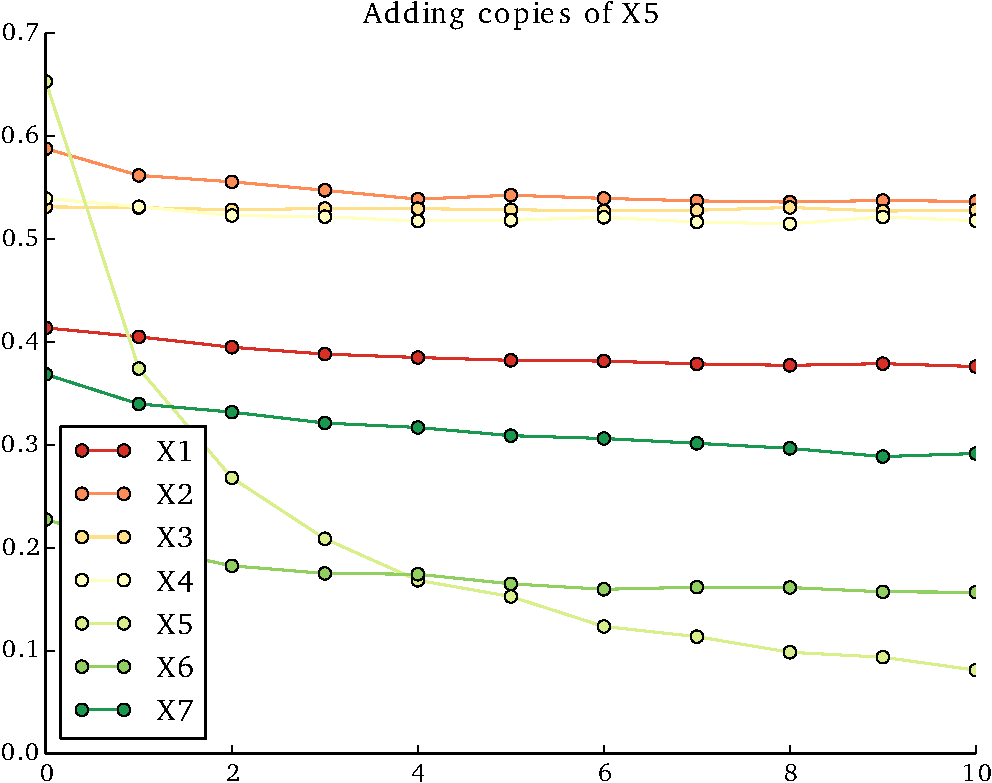
\includegraphics[width=0.9\textwidth]{figures/ch7_red_led.pdf}
\caption{Adding copies of $X_5$ on the LED classification task. The more
         redundant variables are added, the lesser the importance of $X_5$.}
\label{fig:7:red:led}
\end{figure}


\begin{figure}
\centering
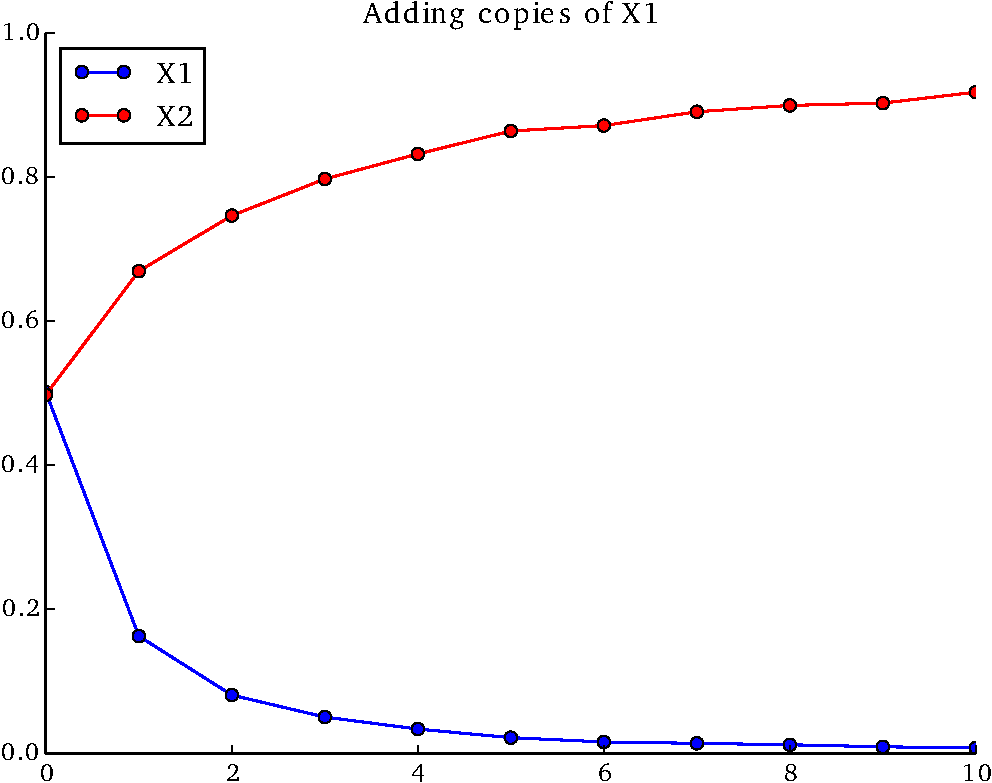
\includegraphics[width=0.9\textwidth]{figures/ch7_red_xor.pdf}
\caption{Adding copies of $X_1$ on a XOR classification task. The more redundant
         variables are added, the lesser the importance of $X_1$, but the larger
         the importance of $X_2$.}
\label{fig:7:red:xor}
\end{figure}

As a second example, Figure~\ref{fig:7:red:xor} illustrates redundancy effects
for a XOR classification problem defined on two variables $X_1$ and $X_2$.
Again, the importance of the duplicated variable $X_1$  decreases as redundant
variables are added, which confirms our results from
Propositions~\ref{prop:red:self} and \ref{prop:red:general}. More
interestingly, we now observe that the importance of the other variable, $X_2$,
increases as copies of $X_1$ are added. For this problem, the
$I(X_2;Y|B,X_1^c)$ terms are prevalent with respect to the $I(X_2;Y|B)$ terms
(which is in fact unique and equal to $0$), thereby artificially increasing the
overall importance of $X_2$ as redundancy augments, as expected from
Propositions \ref{prop:red:other} and \ref{prop:red:general}.

Overall, results presented in this section call for caution when interpreting
variable importance scores. Due to redundancy effects -- either total, as studied
here, or partial as it would often arise in practice -- it may happen that the
total importance of a given variable is either misleadingly low or deceptively
high because the same information is spread within several redundant variables
and therefore taken into account several times within the total importances. As
such, we advise to complement the interpretation with a systematic
decomposition of variable importance scores, e.g., as previously done in
Figure~\ref{fig:decomposition}, in order to better understand why a variable is
in fact important and to possibly detect redundancy.


\section{Bias in variable importances}
\label{sec:7:bias}

In this section, we study sources of bias in variable importances and show that
variable selection (as previously discussed in Section~\ref{sec:ntrt}) is  not
the only cause of bias. In practice, complementary forces due to masking
effects, impurity misestimations and the structure of the trees make variable
importances deviate from the theoretical results found in asymptotic conditions
for totally randomized trees.

\subsection{Bias due to masking effects}

As shown in the previous chapters, the guided selection of the split variable
(i.e., for $K>1$) is necessary for balancing bias and variance in  randomized
decision trees and to produce accurate ensembles. In particular, we studied
that decision trees built with too much randomization usually lead to an
increase of bias which cannot be compensated by a reciprocal decrease of
variance, making it necessary to adjust the value of $K$ to find the
appropriate trade-off. By contrast, we also showed in Section~\ref{sec:ntrt}
that when variable selection is not totally random (i.e., as soon as $K>1$),
masking effects induce a bias with respect to variable importances, since it
forces some of the branches to never be built, and therefore some of the
conditioning sets $B \in {\cal P}(V)$ to never be taken into account. As a
consequence, random forests whose parameter $K$ has been tuned to maximize
accuracy may yield variable importances that are biased (either
over- or underestimated). More specifically, it can be shown (see
Section~\ref{sec:ntrt}) that a relevant variable may be null with regards to
its importance, thereby making it indistinguishable from irrelevant variables,
and that the importance of relevant variables becomes dependent on the number
of irrelevant variables.


\subsection{Bias due to impurity misestimations}
\label{sec:7:bias:high}

In many applications, input variables are heterogeneous and vary in their scale
of measurement or in the number of categories they may take. For example, in
the case of meteorological problems, variables often comprise mixed
environmental measurements of different nature and scale,   like speed of
wind, temperature, humidity, pressure, rainfall or solar radiation. As we show
in this section, misestimations of node impurity is in fact directly
proportional to the cardinality of the split variable and inversely
proportional to the number $N_t$ of samples used for the evaluation. As a
result, impurity reductions become overestimated as we go deeper in the tree
and/or as the number of values of the variable is large. In this context,
variable importances suffer from bias, making variables of higher cardinality
wrongly appear as more important.

To guide our discussion, let us revisit the simulation studies from
\citep{strobl:2007b} which consider a binary output variable $Y$ and five
input variables $X_1,\dots,X_5$, as defined in Table~\ref{table:simulation}.

\begin{table}
    \centering
    \begin{tabular}{| c c c |}
    \hline
    & $X_1$ & $\sim{\cal N}(0, 1)$ \\
    & $X_2$ & $\sim{\cal M}(2)$ \\
    & $X_3$ & $\sim{\cal M}(4)$ \\
    & $X_4$ & $\sim{\cal M}(10)$ \\
    & $X_5$ & $\sim{\cal M}(20)$ \\
    \hline
    \hline
    {\it null case}  & $Y$ & $\sim{\cal B}(0.5)$ \\
    {\it power case} & $Y|X_2=0$ &  $\sim{\cal B}(0.5-\text{relevance})$ \\
                     & $Y|X_2=1$ &  $\sim{\cal B}(0.5+\text{relevance})$ \\
    \hline
    \end{tabular}
    \caption{Input variables are independent random variables as defined from
    the table. ${\cal N}(0, 1)$ is the standard normal
    distribution. ${\cal M}(k)$ is the multinomial distribution with values in $\{0, \dots, k-1\}$
    and equal probabilities. ${\cal B}(p)$ is the binomial distribution. In the
    null case, $Y$ is independent from $X_1, \dots, X_5$. In the power case, $Y$
    depends on the value $X_2$ while other input variables remain irrelevant.}
    \label{table:simulation}
\end{table}

\begin{figure}
\centering
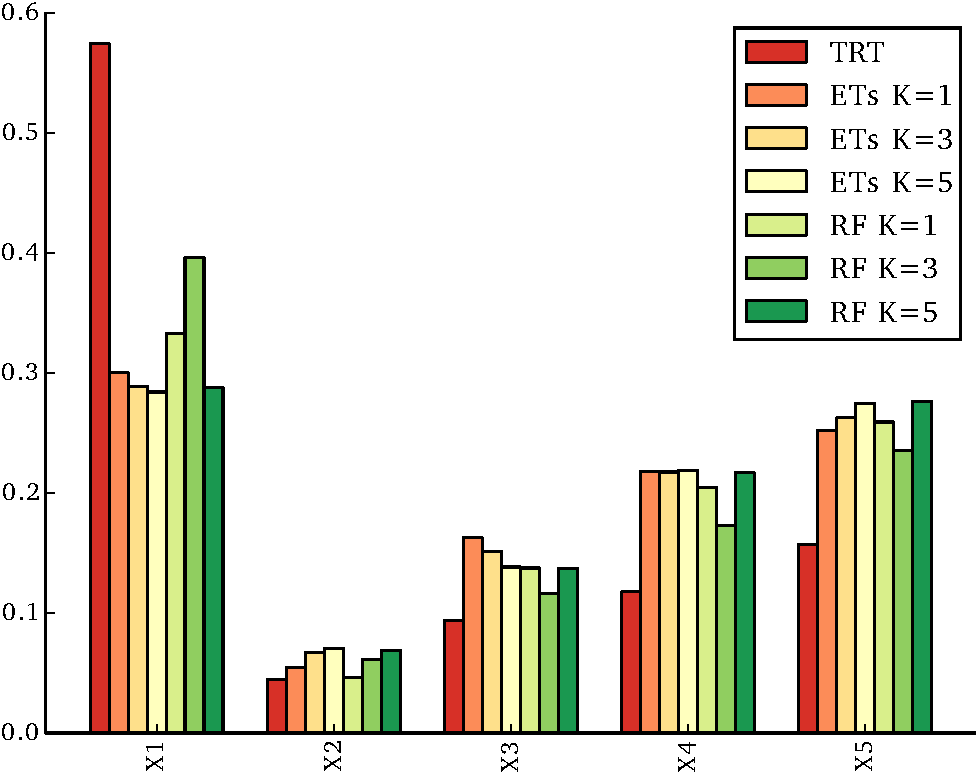
\includegraphics[width=0.9\textwidth]{figures/ch7_bias_null.pdf}
\caption{Variable importances for $Y$ independent of $X_1, \dots, X_5$. ($N=120$, $M=500$)}
\label{fig:7:bias:null}
\end{figure}

Let us first analyze the case where $Y$ is independent from $X_1, \dots, X_5$,
i.e., such that none of the input variables are informative with respect to the
output. For a randomly sampled dataset ${\cal L}$ of $N=120$ samples,
Figure~\ref{fig:7:bias:null} plots variable importances for different kinds of
random forests. TRT corresponds to totally randomized trees, as defined in
Section~\ref{sec:6:theory}, RF corresponds to standard Random Forest with
bootstrap sampling and ETs corresponds to Extremely Randomized Trees. Both RF
and ETs use binary splits while TRT rely on multiway exhaustive
splits\footnote{Thereby creating as many branches as the number of values of
the split variable, even if this variable is continuous and count unique values
only.}. In asymptotic conditions, we proved in Theorem~\ref{thm:irrelevant}
that the importance of irrelevant variables is strictly equal to $0$. For a
finite value of $N$ however, this result does not hold, as
Figure~\ref{fig:7:bias:null} indeed confirms. In contrast with what would be
expected, we observe that the importance of none of the variables is in fact
nowhere close to $0$. In light of Theorem~\ref{thm:sum-of-imp} however, this
result is not that surprising: as long as decision trees can be fully
developed, the sum of variable importances is equal to  the (empirically
estimated) mutual information between $X_1,\dots,X_p$ and the output $Y$, which
is itself upper bounded by the (empirically estimated) entropy $H(Y)$ of the
output variable. In this case, $H(Y)=\log_2(2)=1$, which indeed corresponds to
the sum of variable importances for all methods compared in the figure. More
importantly, we also observe that the larger the cardinality of the variable
(i.e., the larger its number of unique values), the larger its importance. For
example, the importance of $X_1$ (for which samples all have unique values) or
of $X_5$ (which counts up to $40$ unique values) appears nearly $3$ times
larger as the importance of $X_2$ (which is binary).

In their study, \citet{strobl:2007b} argue that this bias is due to variable
selection: \textit{variables with more potential cut-points are more likely to
produce a good criterion value by chance, as in a multiple testing situation}.
As a result, variables of higher cardinality are more likely to be chosen for
splitting than those of lower cardinality. While this bias has been known for
long in decision trees~\citep{kononenko:1995,kim:2001,hothorn:2006}, we argue
that it is not the actual cause for the bias observed here. Indeed, this
argument does not directly explain why similar trends are also observed when no
variable selection is performed (e.g., for TRT or for $K=1$) nor why it
similarly happens when cut-points are chosen at random, independently of the
cardinality of the variable (e.g., in ETs).

For multiway splits like in TRT, bias in variable importances can be traced to the
misestimations of the mutual information terms
\begin{equation}
\Delta i(s, t) \approx I(X_j;Y|t)
\end{equation}
due to the finite size $N_t$ of the node samples. As shown in
\citep{goebel:2005}, when $X_j$ and $Y$ are independent random variables (i.e.,
when $X_j$ is irrelevant), the distribution of finite sample size estimates of
their mutual information  follows approximately a gamma distribution
\begin{equation}
\widehat{I}(X_j; Y) \sim \Gamma\Big( \frac{1}{2}(|{\cal X}_j|-1)(|{\cal Y}|-1), \frac{1}{N_t \log 2} \Big)
\end{equation}
whose mean is linearly proportional to the cardinalities $|{\cal X}_j|$ and
$|{\cal Y}|$ of $X_j$ and $Y$ and inversely proportional to $N_t$:
\begin{equation}
\mathbb{E}\{ \widehat{I}(X_j; Y) \} = \frac{(|{\cal X}_j|-1)(|{\cal Y}|-1)}{2 N_t \log 2}.
\end{equation}
As a result, estimates get larger as $X_j$ counts many unique values, and
become even larger as nodes are deep in the tree (since $N_t$ gets smaller).
Consequently, the weighted mean of all such estimated impurity terms
$I(X_j;Y|t)$, for all nodes $t$ where $X_j$ is the split variable, and
resulting in the total importance $\text{Imp}(X_j)$, is also linearly dependent
on the cardinality of $X_j$. For TRT, this result explains why variables of
high cardinality in Figure~\ref{fig:7:bias:null} appear as more important than
those of lower cardinality. Intuitively, the closer the number of unique values
with respect to the total number of samples, the larger the impurity decrease
when splitting exhaustively on this variable. In the extreme case, when values
for $X_j$ are all unique, splitting on the variable perfectly memorizes the
values of $Y$, resulting in child nodes that are all pure, therefore maximizing
the estimated mutual information. As such, this explains why $X_1$, whose
values are all unique, appears as the most important variable.

For binary splits (i.e., for RF and ETs, but not for TRT) the mutual
information $I(X_j;Y|t)$ is not directly estimated at each node. Rather, in the
case of ordered variables, $\Delta i(s, t)$ corresponds to an estimate of the
mutual information $I(X_j\leq v;Y|t)$ of the binary split $X_j \leq v$. Under
the simplifying assumption that binary splits on the same variable are all
directly consecutive in the decision tree,  it is easy to see that recursive
binary partitioning eventually ends up emulating direct multiway exhaustive
splits, as illustrated in Figure~\ref{fig:7:splits}. Using an argument similar
to the proof of Theorem~\ref{thm:sum-of-imp}, intermediate impurity terms
between the first split and the last of those splits cancel each other when
summing up the importances, which finally amounts to collect an actual estimate
of $I(X_j;Y|t)$ from the sequence of binary splits. For the same reasons as before,
variables of high cardinality are therefore biased in the same way. (As we will
study in Section~\ref{sec:bias:tree}, this assumption does not hold in
practice, making the importances from binary decision trees strictly different
from those of multiway decision trees. Yet, the qualitative conclusions are
still valid since variables of high cardinality can be reused far more many
times than variables of low cardinality, before all possible splits are
exhausted.)

\begin{figure}
    \centering
    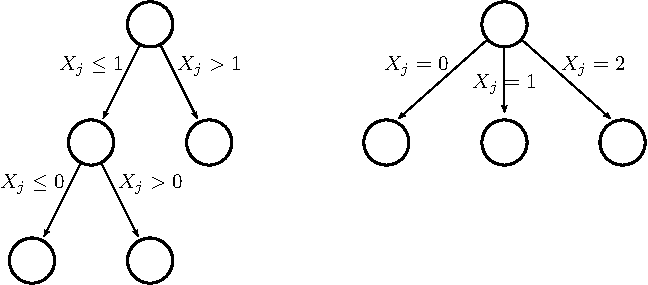
\includegraphics[scale=1.0]{figures/ch7_splits.pdf}
    \caption{Consecutive binary splits on the same variable are equivalent to direct multiway splits.}
    \label{fig:7:splits}
\end{figure}

In both situations, the origin of the problem stems from the fact that node
impurity is misestimated when the size $N_t$ of the node samples is too small.
To a large extent, the issue is aggravated by the fact that trees are fully
developed by default, making impurity terms collected near the leaves usually
unreliable. As a precaution, a safe and effective solution for the bias problem
therefore simply consists in collecting impurity terms only for those nodes
where the impurity estimates can be considered as reliable. Equivalently, the
construction of the tree can also be stopped early, when impurity estimates
become unreliable, e.g., by limiting the depth of the tree, controlling for the
minimum number of samples in internal nodes or using any of the other  stopping
criteria defined in Section~\ref{sec:3:stop}. Among all alternatives,
conditional inference trees~\citep{hothorn:2006} and earlier
methods~\citep{quinlan:1986,wehenkel:1998} make use of statistical tests for
assessing the independence of $X_j$ and $Y$ at a pre-specified level of
confidence $\alpha$. If the null hypothesis cannot be rejected, then recursive
partitioning halts. In particular, variable importances collected from
conditional inference trees were shown experimentally by \citet{strobl:2007b}
not to suffer from bias. The authors argue that it is due to the unbiased
variable selection mechanisms also implemented in conditional inference trees.
By contrast, we argue that the absence of bias in importances from such trees
is mostly due to the early stopping criterion, and not to variable selection.
Although variable selection plays an important and exacerbating role, it is not
the true cause of the  observed bias. Indeed, since the impurity reduction of
variables of high cardinality is overestimated, searching for a split among
$K>1$ randomly drawn variables increases their probability of being selected
when compared to others of lower cardinality, therefore masking and reducing
the importances of these latter variables. Yet, bias stems from the fact
that impurity reductions are misestimated in the first place.

\begin{figure}
\centering
ETs without variable selection\\[1ex]
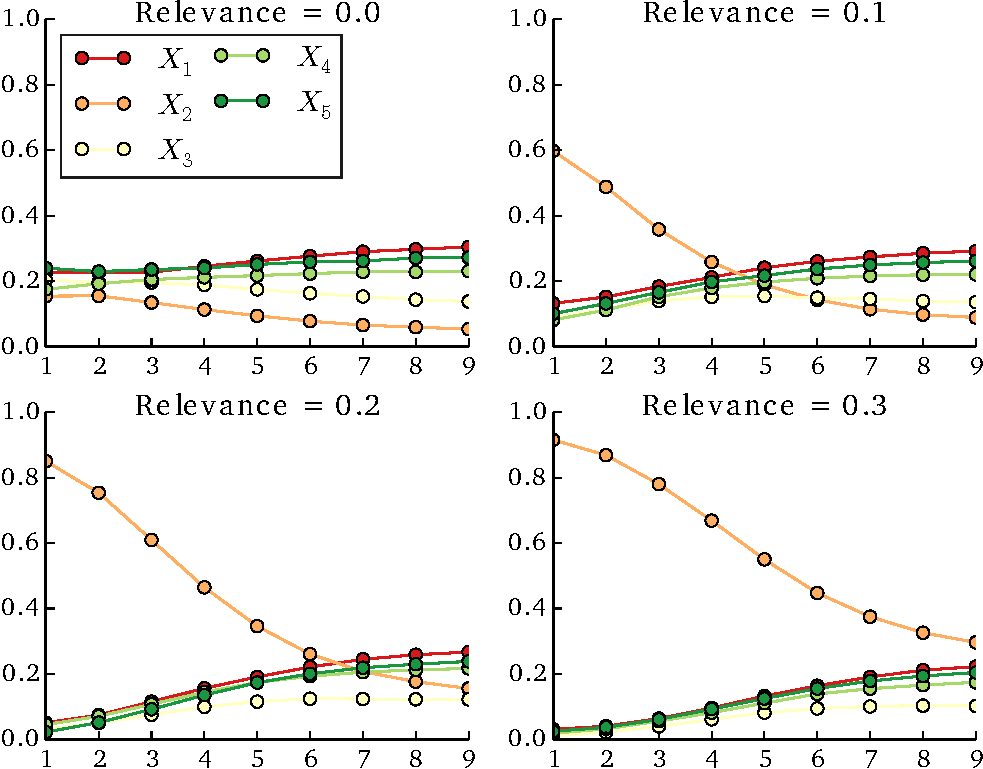
\includegraphics[width=0.9\textwidth]{figures/ch7_bias_depth.pdf}\\[2ex]
Random Forest with variable selection\\[1ex]
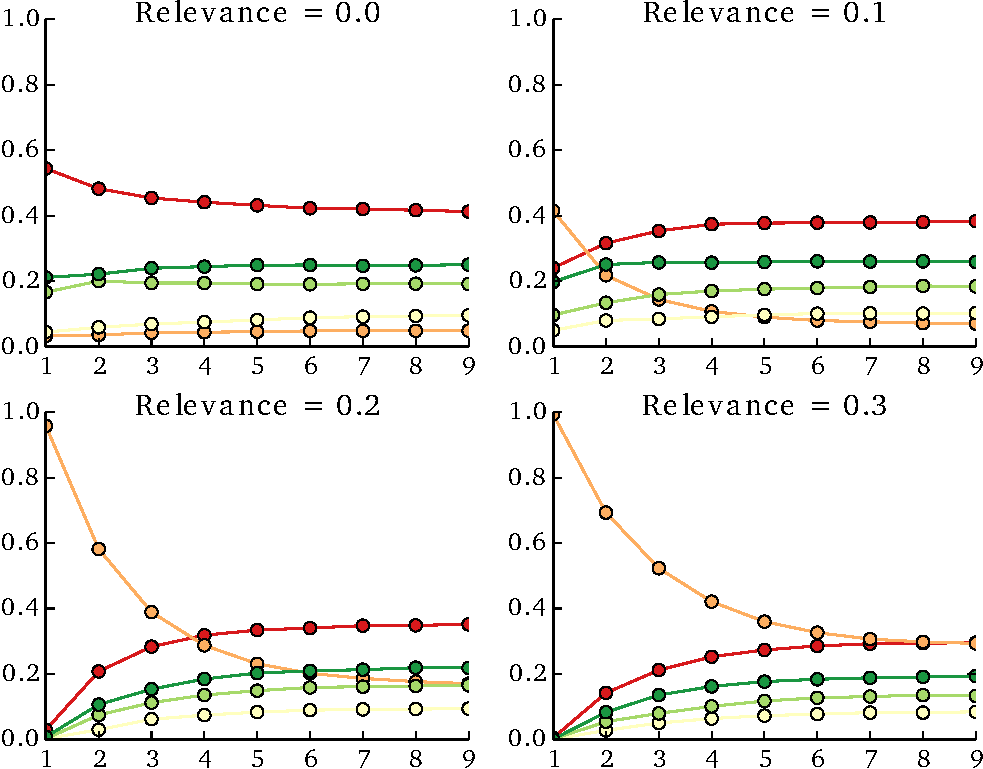
\includegraphics[width=0.9\textwidth]{figures/ch7_bias_depth_rf.pdf}
\caption{Variable importances of $X_1, \dots, X_5$ when varying both the
         maximum depth of the trees and the degree of relevance of $X_2$.
         Importance scores are normalized by the sum of importances.
         (Top) ETs with no variable selection, $K=1$, $N=120$, $M=500$.
         (Bottom) Random Forest with variable selection, $K=5$, $N=120$, $M=500$.}
\label{fig:7:bias:depth}
\end{figure}

As an illustrative example, Figure~\ref{fig:7:bias:depth} reconsiders the
simulation study of Table~\ref{table:simulation}, when varying both the maximum
depth of the trees (from $\texttt{max\_depth}=1$ to $9$) and the relevance of
$X_2$ with respect to $Y$.  Let us first consider ETs  built with no variable
selection ($K=1$), as shown in four top plots of the figure. For the null case,
when $\text{relevance}=0$, limiting the depth of the trees correctly fixes the
bias that was observed before. For shallow trees, the importances before
normalization of all five input variables are close to 0, as expected from
irrelevant variables. The normalized importances, as shown in the figure, are
also all close to $\tfrac{1}{p}=0.2$, confirming that no variable is detected
as more relevant than the others. However, when the depth of the decision trees
increases, importances deviate and bias proportional to the cardinality of the
variables appear as discussed before. When $X_2$ is a relevant variable (i.e.,
for $\text{relevance}>0$), its importance is expected to be strictly positive
and at least as large as the importances of the irrelevant variables. For
$\text{relevance}=0.1$ and $\texttt{max\_depth=1}$, the importance of $X_2$
appears nearly $6$ times larger than the importances of the other variables,
confirming that $X_2$ is correctly identified as a relevant variable.  For
deeper trees  however, noise dominates and the importance of the irrelevant
variables is larger due to misestimations of the impurity terms. As  relevance
increases, $X_2$ can more clearly be identified as a relevant variable. In
particular, the more relevant $X_2$, that is the stronger the signal, the
deeper trees can be built until $X_2$ is made unrecognizable from the
irrelevant variables.

By comparison, the four bottom plots of Figure~\ref{fig:7:bias:depth}
illustrate variable importances for RF built with variable selection ($K=5$).
Again, we observe that limiting the depth of the trees help reduce the
misestimation bias. However, the aggravating effect of variable selection is
also clearly visible: variables of larger cardinality appear as significantly
more important than the other variables. Consequently, this makes the
detection of  $X_2$ as a relevant variable more difficult when trees are grown
deeper. When comparing the relative importance of $X_2$ for a given depth and
relevance, we indeed observe that $X_2$ consistently appears as less important
in RF than in ETs. It is only for very shallow trees ($\texttt{max\_depth=1}$
or $\texttt{2}$) and high relevance that $X_2$ is identified with higher
confidence than in ETs.

In conclusion, evaluating impurity on small samples lead to over-estimations of
the mutual information, resulting in biased variable importances. In
particular, the higher the cardinality of the variable,  the larger the
misestimations. To minimize this effect, caution should be taken by only
considering impurity terms that were computed from a large enough sample. This
can be guaranteed, e.g., by stopping the construction of the tree early, or
making leaves grow more slowly than the size $N$ of the learning set.
Additionally, we have also shown that variable selection may increase the bias
due to over-estimations. In this case, a simple remedy consists in not using
variable selection when assessing the relevance of variables.

\subsection{Bias due to binary trees and threshold selection}
\label{sec:bias:tree}

Previous developments from Chapter~\ref{ch:importances} studied variable
importances for fully developed totally randomized trees and multiway
exhaustive splits. In practice however, random forests usually rely on binary
splits rather than on multiway splits. In terms of impurity, this results in
additional and distinct information terms that were not previously accounted
for, because i) a same variable can be reused several times along the same
branch and ii) binary splits discretize the information contained in a
variable, making variable importances dependent on the split threshold selection
strategy. In lack of a rigorous theoretical framework, we give in this section
preliminary insights on variable importances for binary decision trees,
hopefully shedding some light on their interpretation.

\begin{table}
    \centering
    \begin{tabular}{| c | c c |}
    \hline
    $y$ & $x_1$ & $x_2$ \\
    \hline
    \hline
    0 & 0 & 0 \\
    1 & 1 & 1 \\
    1 & 2 & 1 \\
    \hline
    \end{tabular}
    \caption{Toy problem. All $3$ possible samples are equiprobable.}
    \label{table:simulation:bias:tree}
\end{table}

As a simplistic but illustrative example, let us consider a toy classification
problem composed of a ternary input variable $X_1$ and of a binary input
variable $X_2$, both of them being ordered. Let us further assume that input samples are uniformly drawn
from Table~\ref{table:simulation:bias:tree}, which defines the output as $Y =
X_1 < 1$ and $X_2$ as a copy of $Y$. With respect to $Y$, both variables are as
informative and one should expect their importances to be the same.  With
totally randomized trees and exhaustive splits, two equiprobable decision trees
can be built, as represented in Figure~\ref{fig:7:bias:trees:id3}. In both of
them, splitting either on $X_1$ or on $X_2$ at the root node results in child
nodes that are pure, hence halting the construction process. As expected, the measured
variable importances are the same:
\begin{align*}
\text{Imp}(X_1) &= \frac{1}{2} I(X_1;Y) = \frac{1}{2} H(Y) = 0.459, \\
\text{Imp}(X_2) &= \frac{1}{2} I(X_2;Y) = \frac{1}{2} H(Y) = 0.459.
\end{align*}

\begin{figure}
    \centering
    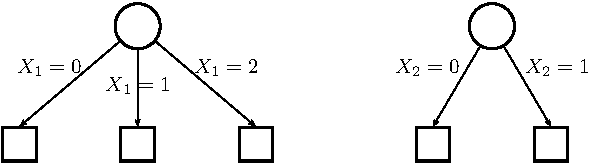
\includegraphics[scale=1.0]{figures/ch7_trees_id3.pdf}
    \caption{Totally randomized trees built from Table~\ref{table:simulation:bias:tree}. Both decision trees are equiprobable. The resulting variable importances indicate that both $X_1$ and $X_2$ are as important. }
    \label{fig:7:bias:trees:id3}
\end{figure}
\begin{figure}
    \centering
    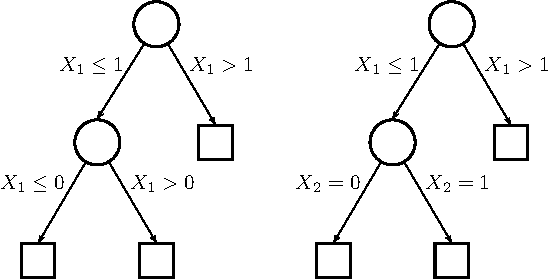
\includegraphics[scale=1.0]{figures/ch7_trees_ets.pdf}\vspace{1cm}\\
    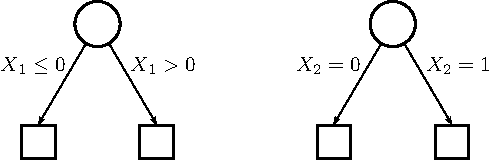
\includegraphics[scale=1.0]{figures/ch7_trees_ets2.pdf}
    \caption{Extremely randomized trees ($K=1$) built from Table~\ref{table:simulation:bias:tree}. From left to right, top to bottom, decision trees are respectively generated with probability $\tfrac{1}{8}$, $\tfrac{1}{8}$, $\tfrac{1}{4}$ and $\tfrac{1}{2}$. The resulting variable importances indicate that $X_2$ is now more important than $X_1$. }
    \label{fig:7:bias:trees:ets}
\end{figure}

By contrast, using binary splits and Extremely Randomized Trees (for $K=1$) results in $4$ different decision trees, as
represented in Figure~\ref{fig:7:bias:trees:ets}. When splitting on $X_1$ at
the root node, two binary splits are now possible with equal probability: $t_L = X_1 \leq 0, t_R = X_1 > 0$ or
$t_L = X_1 \leq 1, t_R = X_1 > 1$. In the former case, the resulting child nodes are pure,
hence halting the construction process. In the latter case, the right child
(corresponding to $X_1 > 1$) is pure, while the left child is not. For this
node, recursive partitioning proceeds and a second binary split can be made either on
$X_1$ or on $X_2$.  Overall, the measured variable
importances in these binary trees, in asymptotic conditions, are
\begin{align*}
\text{Imp}(X_1) &= \frac{2}{8} I(X_1 \leq 1;Y) + \frac{1}{8} P(X_1 \leq 1) I(X_1 \leq 0;Y|X_1 \leq 1) + \frac{1}{4} I(X_1 \leq 0;Y)\\
                &= 0.375 \\
\text{Imp}(X_2) &= \frac{1}{2} I(X_2;Y) + \frac{1}{8} P(X_1 \leq 1) I(X_2;Y|X_1\leq 1)\\
                &= 0.541,
\end{align*}
which makes them strictly different from the importances collected from multiway totally
randomized trees. In particular, due to the binarization of the split
variables, importances now account for conditioning sets that may include
several values of a same variable. For instance, the importance of $X_2$
includes $I(X_2;Y|X_1\leq 1)$, which measures the mutual information between
$X_2$ and $Y$ when $X_1$ is either equal to $0$ or $1$. With multiway
exhaustive splits, these conditioning sets are not considered because branches
correspond to single values only. Similarly, importances also account for
binarized mutual information terms such as $I(X_1 \leq 1;Y)$. Again, these are
not evaluated in totally randomized trees because of the multiway splits.

Accordingly, threshold selection in binary splits has a dominant effect on
variable importances since it controls how the original variables are
binarized. In ETs, all intermediate thresholds $v$ are possible, resulting in a
combinatorial number of additional impurity terms $I(X_j \leq v_j;Y|\cdot)$ and
$I(\cdot;Y|X_j \leq v_j, \cdot)$. In RF, only the best threshold is selected
locally at each node, resulting in fewer additional impurity terms $I(X_j <
v_j^*;Y|\cdot)$ and $I(\cdot;Y|X_j < v_j^*,\cdot)$ (and masking all others).

\begin{figure}
\centering
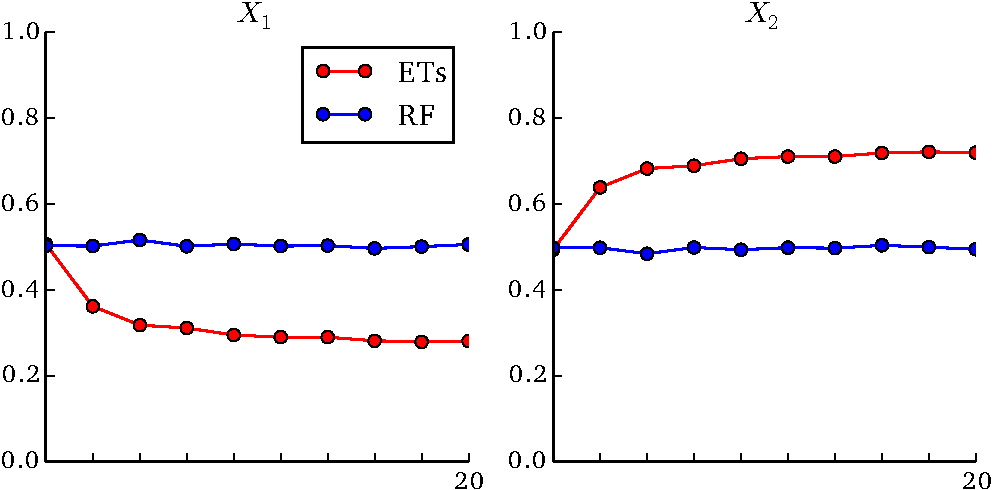
\includegraphics[width=0.9\textwidth]{figures/ch7_bias_trees.pdf}
\caption{Variable importances of $X_1$ and $X_2$ when increasing the cardinality of $X_1$. High cardinality does not necessarily mean high importance. }
\label{fig:7:bias:trees}
\end{figure}

As a last example, Figure~\ref{fig:7:bias:trees} illustrates variable
importances for $X_1$ and $X_2$ when increasing the cardinality of $X_1$ on the
previous toy problem. That is, let us redefine the output as $Y = X_1 <
\tfrac{|{\cal X}_1|}{2}$ while keeping $X_2$ as a binary variable defined as a
copy of $Y$. Assuming that all input samples are equiprobable, the importances
yielded by totally randomized trees with multiway splits remain the same as
before. For ETs however, increasing $|{\cal X}_1|$ induces even more new impurity terms
that are now accounted for in the importances. As the figure shows, increasing
the cardinality of $X_1$ makes its importance decrease, but also simultaneously
makes the importance of $X_2$ increase. Indeed, splitting on $X_2$ always yield
child nodes that are pure, which is unlikely to be the case when splitting
randomly on $X_1$. For RF, only the best thresholds are selected, yielding in
this case child nodes that are always pure, as for totally randomized trees.
As such, their importances respectively appear as equal as the figure confirms.

Overall, these additional effects due to binary splits make variable
importances computed from classical random forests very difficult to interpret
and understand, as soon as data include many variables of different scale
or number of categories. While they can still be
used to identify the most relevant variables, caution should be taken when
interpreting the amplitude of importance measures. As our last example
illustrates, the importance of a variable may be misleadingly low or
misleadingly high because of combinatorial effects, solely due to the possible
ways variables are binarized.

\begin{remark}{Encoding $N$-ary variables into binary variables}
Partitioning node samples with binary splits on $N$-ary input variables is
equivalent to individually transforming each input variable $X_j$ into a set of
$b_j$ binary input variables $\{X_j^{m} | m=1,\dots,b_j\}$, each encoding for
one the possible splits, and then partitioning node samples using of one these new
variables. If we consider the binarized learning set ${\cal L}^\prime$, for
which all $p$ the input variables have been transformed into $\sum b_j$ binary
variables, then our theoretical framework for totally randomized trees and
exhaustive splits can be applied and Theorem~\ref{thm:imp} could possibly be
adapted. The only difference lies in the way binary variables are drawn at
random:  instead of splitting randomly on one of the $\sum b_j$ variables,
first, one of the $p$ original variables is drawn uniformly at random; second, one of
its $b_j$ binary variables is selected for splitting the current node. In this
setting, the importance of $X_j$ therefore amounts to the sum of importances $\sum
\text{Imp}(X_j^m)$ of its binary variables. \end{remark}


\section{Applications}
\label{sec:7:applications}

In spite of the various concurrent effects discussed earlier, variable importance
measures have been used with success in a wide range of scientific
applications.  While  they have proven to be a good proxy for assessing the
relevance of input variables, providing helpful insights, too often variable
importances are used as a black-box metric, hence under-exploiting the
information they offer. As such, examples presented in this section all
demonstrate that any progress towards a better theoretical understanding of
variable importances may help to further advance a wide range of research
domains.

\subsection{Feature selection}

Within the past 10 or 20 years, typical machine learning problems have
grown from a few tens of input variables to domains exploring hundreds of
thousands of variables, often comprising noisy, irrelevant or redundant
predictors, mixing both numerical and categorical variables and involving
complex interaction effects. In this context, the feature selection problem
consists in identifying a subset of the original input variables that are
useful for building a good model~\citep{guyon:2003,liu:2005}. The
advantages and benefits of reducing the dimensionality of the problem
include: speeding up machine learning algorithms, reducing measurement and
storage requirements, improving the accuracy of the models or facilitating
data visualization and understanding.

Because of the properties of random forests (good prediction performance,
robustness to noisy variables, support of numerical and categorical
variables and ability to model complex interactions), variable importances
often provide an effective solution for the feature selection problem. The
most straightforward solution consists in ranking variables according to
their importance scores and to only keep the most important ones. Depending
on the objective, the best subset of variables can be identified in
several ways:

\begin{itemize}
\item  When the goal is simply to reduce dimensionality because of speed
       and storage requirements, the simplest solution
       is to keep only those variables whose importances $\text{Imp}(X_j)$
       is greater than some manually defined threshold $\alpha$.

\item If the goal is to improve accuracy, a good subset
      of variables can typically be found by tuning the threshold $\alpha$ so
      as to minimize some user-defined criterion (e.g., the zero-one loss in
      classification or the squared error loss in regression) for the model
      built on the subset $\{X_j | \text{Imp}(X_j) > \alpha \}$.

      At the price of more computational efforts, even better performance can
      usually be reached by embedding variable importances into a dedicated
      iterative feature selection procedure, such as those described in
      \citep{guyon:2002,tuv:2009}.

\item In some other applications, the objective is to identify variables
      that are relevant, in order to better understand the underlying relations
      with the output $Y$. In asymptotic conditions, this could be done by
      discarding all variables whose importances is null, as shown by
      Theorem~\ref{thm:relevant}. In a finite setting however, bias due to
      masking effects or impurity misestimations (as previously discussed in
      Section~\ref{sec:7:bias}) makes it more difficult to identify variables
      that are truly relevant since their importances might appear to be lower
      than those of irrelevant variables. Yet, several options are available
      for controlling and limiting false positives, such as stopping the
      construction process when impurity estimations become statistically
      unreliable (Section~\ref{sec:7:bias:high}), comparing the importances of
      the original input variables to artificial contrasts \citep{tuv:2006} or
      robustly controlling the conditional error rate through permutation tests
      \citep{saeys:2012}.

\end{itemize}


\subsection{Biomarker identification}

With the rise of \textit{-omics} data, random forests have become one of the
most popular tools in life sciences, providing practitioners with both
high-prediction accuracy and helpful insights about the importances of variables. In
many cases, variable importance measures (either MDI or the permutation
importance) is exploited to better understand the complex interaction effects
between the inputs and the output. Examples of successful applications include
the identification of risk-associated SNPs in genome-wide association studies
\citep{lunetta:2004,meng:2009,botta:2014}, the discovery of important genes and
pathways from micro-array gene-expression data \citep{pang:2006,chang:2008} or
the identification of factors for predicting protein-protein
interactions~\citep{qi:2006}. These examples are not isolated and tens of
further studies based on random forests could in fact be cited from the fields
of genomics, metabolomics, proteomics or transcriptomics. Some of them are
reviewed in \citep{touw:2013,boulesteix:2012}.

In light of our study and discussion of variable importances,  recommendations
for biomarker identification depend on the exact objective of the application.
If the goal is to identify all relevant variables, then totally randomized
trees with multiway splits should be preferred. They indeed constitute the only
method for which variable importances are unbiased, taking into account all
possible interaction terms in a fair and exhaustive way. The only caveat is
that a (very) large number of trees may be required before variable importances
converge, making them computationally intensive to compute, even if the full
randomization of the induction procedure actually make individual decision
trees to be quite fast to generate.  By contrast, if the objective is only to
identify a subset of good predictors for predicting the output (hence possibly
omitting relevant but redundant variables), then non-totally randomized trees
(e.g., standard RF or ETs) with $K$ chosen to maximize accuracy should be
preferred. Even if some informative variables may be masked because of variable
selection, a good subset of input variables should still be identifiable from
importance scores. From a computational point of view, convergence should also
be faster, making this approach more appealing when resources are limited. In
all cases, impurity misestimations should be controlled by stopping the
construction process early or collecting importances only for those nodes where
impurity reductions can be considered as reliable. Finally, whenever practical,
variable importances should also be decomposed in order to better understand
why some variables appear as more important than others. In particular,
studying the decomposition might help identify redundancy effects.

\subsection{Network inference}

Given a set of input variables $V = \{X_1,\dots,X_p\}$, the \textit{network
inference} problem consists in the identification of conditional dependencies
between variables. In genomics for example, regulatory network inference
consists in the identification of interactions between genes or transcription
factors on the basis of their expression level, in order to reconstruct a global
network of interactions (as illustrated in Figure~\ref{fig:7:network} for
Staphylococcus aureus).

\begin{figure}
\centering
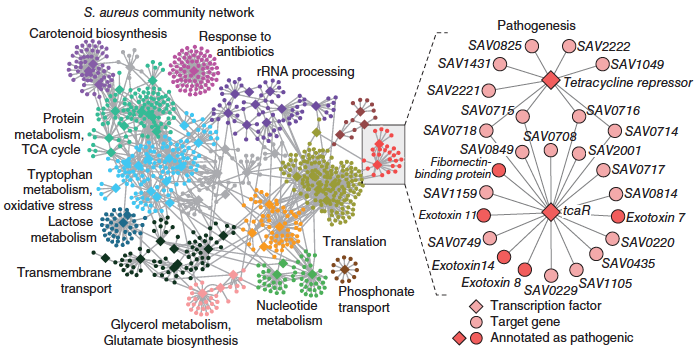
\includegraphics[width=0.9\textwidth]{figures/ch7_network.png}
\caption{Gene regulatory network in Staphylococcus aureus. Image from \citep{marbach:2012}.}
\label{fig:7:network}
\end{figure}

As proposed in the GENIE3 method~\citep{irrthum:2010}, the network inference
problem can be solved generically by remarking  that it can decomposed into $p$
independent supervised learning problems. Formally, for each input variable
$X_j$ (for $j=1,\dots,p$), GENIE3 considers the supervised sub-problem
consisting in the prediction of the target variable $X_j$ from the remaining
$p-1$ variables $V^{-j}$. Using random forests for solving each of these $p$
problems, variable importances can be derived and used as an indication of the
putative link with $X_j$. Intuitively, the larger the importance, the more
likely the conditional dependency with $X_j$. Once all $p$ problems are solved,
putative links are aggregated over all $p$ variables to provide a ranking of
interactions from which the network can finally be reconstructed.

Again, our previous theoretical analysis call for caution when plugging
variable importances into network inference procedures. Since the goal is to
retrieve all interactions, variable importances should be as unbiased as
possible, which is guaranteed using totally randomized trees with multiway
splits. When input variables are of different scale of measurements or vary in
the number of categories, care should also be taken when aggregating variable
importances into a single ranking of interactions. As shown by Theorem~\ref{thm:sum-of-imp},
variable importances are in this case upper bounded by the entropy $H(X_j)$ of the target variable,
which may greatly varies from one target to another. As such, variable
importances are not directly comparable and should preferably be normalized (e.g., by
$H(X_j)$) before their aggregation. Finally, the use of variable
importances for network inference might not be as appropriate as desired when looking
\textit{direct} interactions since they also account for indirect and combined effects.
In this case, a better strategy might be to look for \textit{strongly} relevant
variables, that is for variables $X_i$ such that $I(X_i;X_j|B) > 0$ for \textit{all} $B$.


% use trt
% mixed input variables => normalize by H(X_j)
% direct verus indirect interations
